% nastavenia prostredia
\documentclass[12pt,a4paper,titlepage,final]{report}
\usepackage[utf8]{inputenc}
\usepackage[T1, IL2]{fontenc}
\usepackage{graphicx}
\usepackage{epstopdf}
\usepackage[margin=2cm]{caption}
\usepackage[top=3cm, left=2cm, right=2cm, text={17cm, 24cm}, ignorefoot]{geometry}
\usepackage{color}
\usepackage{url}
\usepackage[bookmarksopen,colorlinks,plainpages=false,urlcolor=blue,unicode]{hyperref}
\usepackage{setspace}
\usepackage[czech]{babel}
\singlespacing

\begin{document}
	% define
	\def\authora{Jan Bureš}
	\def\authorb{Pavel Macenauer}
	\def\emaila{xbures19@stud.fit.vutbr.cz}
	\def\emailb{xmacen02@stud.fit.vutbr.cz}
	\def\docname{Počítačová grafika}
	\def\projname{Raytracing na CUDA}
	% titulna strana
	\begin{titlepage}

\vspace*{1cm}

\begin{figure}
  \centering
  
\includegraphics[height=6cm]{images/fit.pdf}
\end{figure}

\vspace*{5mm}

\begin{center}
\begin{Large}
Projekt do předmětu PGR -- Počítačová grafika
\end{Large}
\end{center}

\vspace*{5mm}

\begin{center}
\begin{Huge}
CUDA Raytracer \\
\end{Huge}
\end{center}

\vspace*{1cm}

\begin{center}
\begin{Large}
\today
\end{Large}
\end{center}

\vfill

\begin{flushleft}
\begin{large}
\begin{tabular}{ll}

\bf Řešitelé:\hspace{3mm}
& Jan Bureš (\verb_xlogin00@stud.fit.vutbr.cz_) \\
& Pavel Macenauer (\verb_xmacen02@stud.fit.vutbr.cz_) \\
& Fakulta Informačních Technologií \\
& Vysoké Učení Technické v~Brně

\end{tabular}
\end{large}
\end{flushleft}

\end{titlepage}

% vim:set ft=tex expandtab enc=utf8:

	% kapitoly
	\newpage
	\pagestyle{plain}
	\pagenumbering{arabic}
	\setcounter{page}{1}
	\setcounter{secnumdepth}{-1}
	\setlength{\parindent}{1cm}	

%---------------------------------------------------------------------------
\section{Zadání}

\begin{itemize}
	\item Implementace Raytraceru pomocí technologie CUDA v následujícím rozsahu:
	\begin{itemize}
		\item Geometrická primitiva: roviny, koule
		\item Phongův osvětlovací model
		\item Bodové zdroje světla a stíny
		\item Odlesky
	\end{itemize}
	\item Akcelerace výpočtu scény
	\begin{itemize}
		\item průzkum akcelerace raytracingu na GPU
		\item subsampling
		\item využití akcelerační struktury pro výpočet (BVH, KD-tree, octree, ...)
	\end{itemize}
	\item Vygenerování demonstrační scény a její vykreslení
\end{itemize}

%---------------------------------------------------------------------------
\section{Použité technologie}

\subsection{Technologie potřebné pro spuštění programu:}
\begin{itemize}
	\item CUDA 3.0
	\item OpenGL 4
	\item GLM
	\item Glut
	\item Glew
\end{itemize}
\subsection{Při tvorbě jsme použili tyto programy:}
\begin{itemize}
	\item Visual Studio 2012 + NSight
	\item GitHub
\end{itemize}
%---------------------------------------------------------------------------
\section{Použité zdroje}

\subsection{Studijní zdroje:}
\begin{itemize}
	\item Přednáška PGR (Realistické zobrazování I - Ray Tracing)
	\item \href{https://www.fit.vutbr.cz/study/courses/PGR/private/Aurelius.zip}{Ray-tracer Aurelius}
	\item Přednáška PGP (Fotorealistcké zobrazování, optimalizace sledování paprsku)
	\item \href{http://docs.nvidia.com/cuda}{CUDA Toolkit Documentation}
\end{itemize}

\subsection{Doplňujicí zdroje:}
\begin{itemize}
	\item \href{http://cs.wikipedia.org/wiki/Phong%C5%AFv_osv%C4%9Btlovac%C3%AD_model}{Phongův osvětlovací model}
	\item \href{http://stackoverflow.com/questions/19013156/how-does-cuda-4-0-support-recursion}{Rady ohledně rekurze v CUDA}
	\item \href{http://www.3dmuve.com/3dmblog/?p=182}{Bounding Volume Hierarchies (BVH) – A brief tutorial on what they are and how to implement them}
	\item \href{http://cuda-programming.blogspot.cz/2013/01/what-is-constant-memory-in-cuda.html}{What is constant memory in CUDA?}
	\item \href{http://cg.alexandra.dk/2009/08/10/triers-cuda-ray-tracing-tutorial/}{Triers CUDA ray tracing tutorial}
\end{itemize}
%---------------------------------------------------------------------------
\section{Nejdůležitější dosažené výsledky}

\subsection{Scéna}
\begin{itemize}
	\item 50 koulí
	\item 4 roviny
	\item 1 lesklý materiál
	\item 1 bodové světlo
\end{itemize}

\begin{center}

	\captionsetup{type=figure}
		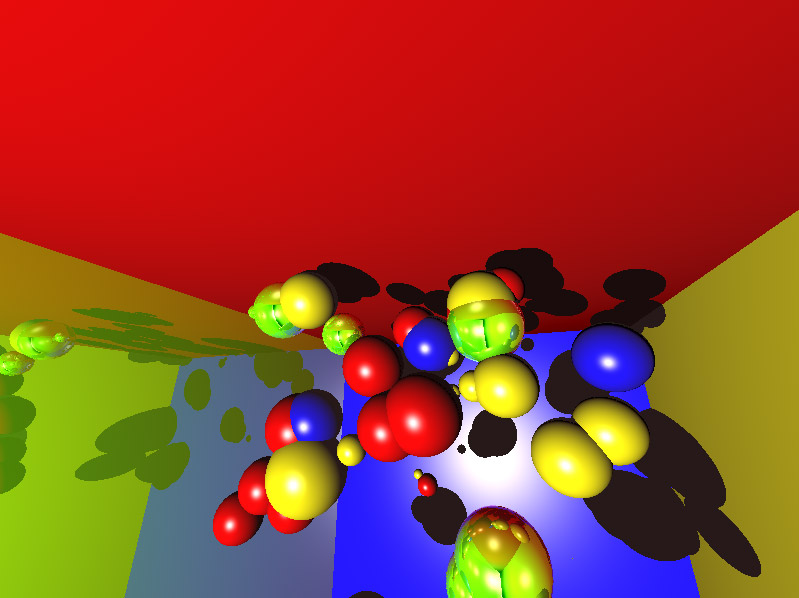
\includegraphics[width=14cm]{images/no-sampling-no-bvh.jpg}
	\captionof{figure}{Vygenerovaná scéna bez využití jakéhokoliv urychlení}
	

	\captionsetup{type=figure}
		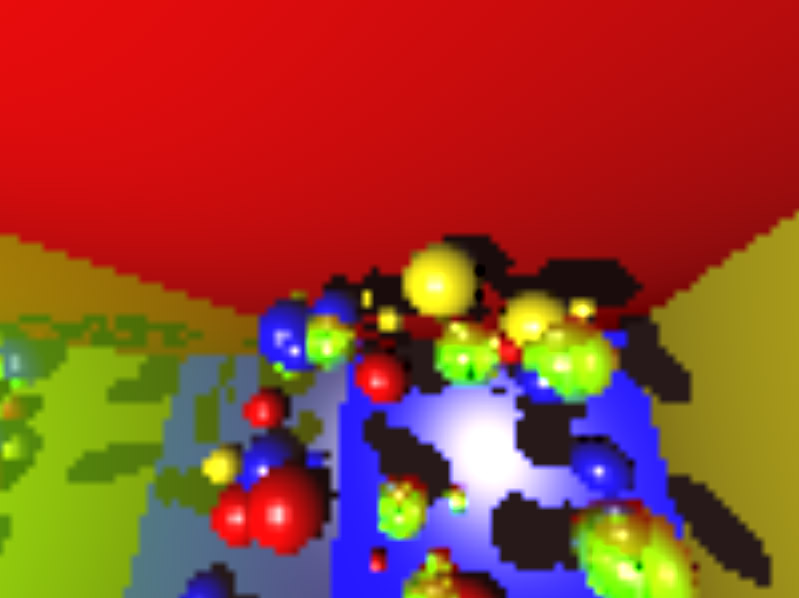
\includegraphics[width=14cm]{images/with-sampling-no-bvh.jpg}
	\captionof{figure}{Vygenerovaná scéna s využitím bilineární samplování}
\end{center}
	\vspace{5mm}
Jedním z nápadů jak urychlit běh programu výpočtu bylo využít vzorkování/samplingu. Při výpočtu se inicializuje paprsek a následně výpočetní vlákno (thread) pro každý obrazový bod, jejich počet je tak roven ŠÍŘKA OBRAZU * VÝŠKA OBRAZU. 
	
	Při klasickém raytracingu na CPU, lze urychlit běh programu tak, že se nevyšle takto paprsek pro každý bod, ale třeba jen pro každý 8-smý a v případě, že paprsek trefí stále stejné primitivum, tak se barvy mezi těmito body interpolují. V opačném případě se pak vyšlou paprsky pro všechny body neb se jedná o rozhraní mezi 2-mi primitivy.
	
	Na GPU je ten problém, že veškeré výpočty probíhají paralelně a jakékoliv podmínky dramaticky snižují výkonnost. Není tak jednoduše možné říct, kdy vyslat všechny paprsky a kdy jen některé, protože se paprsky posílají po skupinách. Optimalizaci jsme tak provedli pomocí bilineárního samplování, kdy ve směru jak osy X, tak osy Y vyšleme počet paprsků dělený předem danou konstantou (na Obrázku 2. je hodnota konstanty 8), čímž snížíme počet výpočetních vláken druhou mocninou konstanty.
	
	Vypočtené hodnoty následně uložíme do sdílené paměti v rámci jednoho warpu a pro celý obraz hodnoty dopočteme pouze z těchto vzorků. Výsledný obraz je však výrazně nižší kvality, než-li obraz vygenerovaný bez použití samplování.


\subsection{Měření na NVidia Quadro K1000M}
\begin{itemize}
	\item CUDA Processing cores: 192
	\item Memory: 2 GB
	\item Memory bandwidth: 29 GBps 
\end{itemize}	
	
\begin{table}[h!]
	\begin{center}
    \begin{tabular}{ | p{3.5cm} | p{3.5cm} | p{3.5cm} | p{3.5cm} |}
    \hline
    Rozlišení & Prům. doba běhu kernelu bez BS [s]& konst=4 [s]& konst=8 [s]
    \\ \hline
    
	1600x800 & 0.1065 & 0.0199 & 0.0068
	\\ \hline
	
	800x600 & 0.0495 & 0.0070 & 0.0030
	\\ \hline
	
    \end{tabular}
	\end{center}	
	\caption{Doba běhu kernelu}  
\end{table}


%---------------------------------------------------------------------------
\section{Ovládání vytvořeného programu}

Program se spustí přes RayTracer.exe s tím, že v konzoli se vypisují hodnoty doby výpočtu kernelu v sekundách.

Při kompilaci lze zapnout/vypnout v souboru \verb|constants.h| parametry se kterými se scéna vypočítává:
\begin{itemize}
	\item \verb|NUM_SPHERES| počet koulí ve scéně pro zvýšení komplexity
	\item \verb|BILINEAR_SAMPLING| využití bilineárního samplování
	\item \verb|SUB_CONST| konstanta, kterou se redukuje počet vláken při bilineárním samplování
	\item \verb|USE_BVH| využití Bounding Volume Hierarchy
\end{itemize}

%---------------------------------------------------------------------------
\section{Zvláštní použité znalosti}

V podstatě všechny vědomosti, které jsme museli nastudovat ohledně architektury CUDA, programovani a debugováni CUDY v prostředí Visual studio 2012 a NVIDIA Nsight.

%---------------------------------------------------------------------------
\section{Rozdělení práce v týmu}

\begin{itemize}
\item xbures19: Phongův osvětlovací model, úprava bilinear sampling, část raytraceru 
\item xmacen02: Základní kostra programu, optimalizace využitých paměťových jednotek, bilinear sampling, část raytraceru 
\end{itemize}

%---------------------------------------------------------------------------
\section{Co bylo nejpracnější}

Popište, co vám při řešení nejvíce komplikovalo život, s čím jste se museli
potýkat, co zabralo čas.

Rozsah: 5-10 řádků

Na celé práci bylo asi nejložitější upravit algoritmus sledování paprsku tak,
aby fungoval na architektuře CUDA. Dále pak správné rozdělení vláken do warpů 
a rozhodnout, který druh paměti použít pro které proměnné. Mno času bylo zapotřebí  
také věnovat rekurzi, kterou by sice CUDA měla podporovat od verze 3.0,  
ovšem stále program havaroval kvůli přetečení zásobníku.

%---------------------------------------------------------------------------
\section{Zkušenosti získané řešením projektu}

Popište, co jste se řešením projektu naučili. Zahrňte dovednosti obecně
programátorské, věci z oblasti počítačové grafiky, ale i spolupráci v týmu,
hospodaření s časem, atd.

Rozsah: formulujte stručně, uchopte cca 3-5 věcí

Naučili jsme se více o architektuře CUDA, vyzkoušeli si implementovat phongův osvětlovací model a
raytracer. Dále jsme si prostudovali možné algoritmické optimalizace raytraceru a některé znich implementovali.

%---------------------------------------------------------------------------
\section{Autoevaluace}

\paragraph{Technický návrh (85\%):} (analýza, dekompozice problému, volba
vhodných prostředků, $\ldots$) 
Tvorbu programu jsme si před implementací dobře rozmysleli a až na pár úprav nebylo nutné přepisovat již implementované části.

\paragraph{Programování (75\%):}
Kód je dobře strukturováný, ale mohl by být více okomentován. 
Implementovaný raytracer je možné dále rozšiřovat a upravovat.

\paragraph{Vzhled vytvořeného řešení (80\%):} 
Scéna vypadá docela pěkně. Některé optimalizace kvalitu mírně zhorší, ale vždy dle očekávání.

\paragraph{Využití zdrojů (90\%):}
Hodně jsme využil již implementovaný raytracer. Trochu méně jsme pak použiváli dostupnou literaturu.

\paragraph{Hospodaření s časem (70\%):}
Začali jsme docela brzo. Uprostřed náše snaha mírně opadla kvůli jiným povinnostem ve škole. Na závěr jsme se snažili vše dokončit.

\paragraph{Spolupráce v týmu (95\%):}
Od začátku jsme komunikovali ohledně podmínek spolupráce. Následné programování pak probíhalo bez problémů.

\paragraph{Celkový dojem (90\%):} (pracnost, získané dovednosti, užitečnost,
volba zadání, cokoliv, $\ldots$)
Stručně (5-10 řádků) komentujte hodnocení.
Celý projekt se nám jevil mírně obtížnější vzhledem k ostatním projektům na škole. 
Nicméně získané vědomosti a zkušenosti jsou určitě přínosem. 
Vybrali jsme si téma projektu kvůli architektuře CUDA, kterou jsme si díky tomuto projektu přiblížili. 
Celý projekt byl zajímavý také tím že jsme si vyzkoušeli vytvořit aplikaci uplně od začátku. 
%---------------------------------------------------------------------------
\section{Doporučení pro budoucí zadávání projektů}

Co vám vyhovovalo a co nevyhovovalo na organizaci projektů? Které prvky by měly
být zachovány, zesíleny, potlačeny, eliminovány?
Do budoucna by určitě bylo vhodné mírně specifikovat požadavky k zadanému tématu (např. 5 odrážek). 

%---------------------------------------------------------------------------

\end{document}
% vim:set ft=tex expandtab enc=utf8:
